\documentclass{article}
\usepackage{zeta}
\usepackage{graphicx}

% the tables are wide
\topmargin=0pt
\oddsidemargin=-0.25in
\evensidemargin=-0.25in
\textwidth=6.5in
\textheight=8.5in

% table of requests
\newenvironment{reqtab}[2]{%
\begin{table}%
\centering
\caption{#2}%
\label{table-#1}%
\begin{tabular}{rll}%
\multicolumn{1}{c}{\bf name}&%
\multicolumn{1}{c}{\bf request}&%
\multicolumn{1}{c}{\bf meaning}\\\hline
}{\end{tabular}%
\end{table}}

% table of responses
\newenvironment{resptab}[2]{
\begin{table}%
\centering
\caption{#2}%
\label{table-#1}%
\begin{tabular}{rll}%
\multicolumn{1}{c}{\bf name}&%
\multicolumn{1}{c}{\bf response}&%
\multicolumn{1}{c}{\bf meaning}\\\hline
}{\end{tabular}%
\end{table}}
% tokens
\newcommand{\stok}[1]{{$\langle${\em #1}$\rangle$}}
\newcommand{\bfid}[1]{{\bf #1}}
\newcommand{\itid}[1]{{\it #1}}

\title{A Networked {\em Gothello} Referee: Specification}
\author{Bart Massey}

\begin{document}
\maketitle

{\em Gothello} is a
game of skill created by the author for
educational purposes. It is played on an ordinary
checkerboard, and has something of the feel of Othello or
Go.  In this document, we will describe a networked server
to which human and computer Gothello players can connect to play
the game in a refereed fashion.

\section{The Game Of {\em Gothello}}

The rules of Gothello are intended to capture some of the
feel of Go, while being more amenable to adversary search.
Gothello is a two player game, played by players conventionally
designated as {\em black} and {\em white}.
\begin{zed}
PLAYER ::= black | white
\end{zed}
\begin{axdef}
  opponent : PLAYER \bij PLAYER
\where
  opponent~white = black \\
  opponent~black = white
\end{axdef}

The board,
shown in figure \ref{fig-board}, is an ordinary
checkerboard or go board: black and white stones are placed on
intersections
(conventionally designated using standard algebraic
notation).  For the purposes of this document, the game
will be played with a 5x5 array of intersections.
\begin{zed}
DIGIT == 1 \upto 5 \\
SQUARE == DIGIT \cross DIGIT
\end{zed}
At any given point in the game, the board position can
be given by noting whether each square is blank or
contains a colored stone.
\begin{zed}
SQUAREVAL ::= stone \ldata PLAYER \rdata | blank \\
BOARD == SQUARE \fun SQUAREVAL
\end{zed}
\begin{schema}{GothelloPosition}
  board : BOARD \\
  to\_move : PLAYER
\end{schema}
The board begins empty, and black moves first.
\begin{schema}{InitGothelloPosition}
  GothelloPosition '
\where
  board' = SQUARE \cross \{ blank \}
\also
  to\_move' = black
\end{schema}

\begin{figure}
\begin{center}
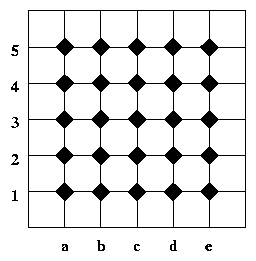
\includegraphics[width=4in]{gothello-board-empty.png}
\end{center}
\caption{Gothello Board In Initial Configuration}
\label{fig-board}
\end{figure}


The players alternate in placing stones of their own color
on blank spaces on the board.  Stones of the same
color which are connected horizontally and/or vertically
are {\em neighbors}.
\newcommand{\adjoins}{\Zinrel{adjoins}}
\begin{zedgroup}
\begin{zdirectives}
\zrelation{(\_\adjoins\_)}
\end{zdirectives}
\begin{axdef}
  \_ \adjoins \_: SQUARE \rel SQUARE
\where
  (\_ \adjoins \_) = \\
  \t1 \{ d, d_1, d_2: DIGIT | d_2 = d_1 + 1 @
         ((d_1, d), (d_2, d)) \}~\cup \\
  \t1 \{ d, d_1, d_2: DIGIT | d_2 = d_1 + 1 @
         ((d, d_1), (d, d_2)) \}
\end{axdef}
\end{zedgroup}
\begin{axdef}
  neighbor: BOARD \fun (SQUARE \rel SQUARE)
\where
  \forall board: BOARD @ \\
  \t1 neighbor~board = \{ s_1, s_2: SQUARE |
        s_1 \adjoins s_2 \land \\
  \t2   board~s_1 \neq blank \land
        board~s_1 = board~s_2 \}
\end{axdef}
A maximal set of mutual neighbors is a {\em group}.
It is most useful to talk about the group containing some
specific board position in a given board.
\begin{axdef}
  group: BOARD \fun SQUARE \fun \power SQUARE
\where
  \forall board: BOARD; s: SQUARE | board~s \neq blank @ \\
  \t1 group~board~s = (neighbor~board)\plus\limg \{s\} \rimg
\end{axdef}

The other key concept in the rules is the concept of
liberties of a group.  These are the blank squares
immediately surrounding the group.  The liberties of
a position are the liberties of the group at that position.
\begin{axdef}
  adjoining\_squares: \power SQUARE \fun \power SQUARE \\
  group\_liberties: BOARD \fun \power SQUARE \fun \power SQUARE \\
  liberties: BOARD \fun SQUARE \fun \power SQUARE
\where
  \forall ss: \power SQUARE @ \\
  \t1 adjoining\_squares~ss =
      (\_ \adjoins \_)\limg ss \rimg \setminus ss
\also
  \forall board: BOARD; ss: \power SQUARE @ \\
  \t1 group\_liberties~board~ss =
      adjoining\_squares~ss \cap
      board\inv\limg \{ blank \} \rimg
\also
  \forall board: BOARD @ \\
  \t1 liberties~board = (group\_liberties~board) \circ (group~board)
\end{axdef}



There are a number of possible outcomes of a player's
turn.
\begin{zed}
  RESULT ::= win \ldata PLAYER \rdata | draw | not\_done | illegal\_move
\end{zed}

A player may pass on any turn, and must pass if
no legal move is available.  The game is over when
both players have passed in succession. This is
a function of the immediate history of the game
({\it i.e.\/}, the sequence of moves that have been made
recently).
\begin{zed}
  MOVE ::= move \ldata SQUARE \rdata | pass \\
  HISTORY == \seq MOVE
\end{zed}
\begin{schema}{GothelloGame}
  GothelloPosition \\
  history: HISTORY
\end{schema}
\begin{schema}{InitGothelloGame}
  InitGothelloPosition \\
  history': HISTORY
\where
  history' = \emptyset
\end{schema}

In short, when the Gothello referee receives an action, it
gets a move, records it in the history, and
report the result.
\begin{schema}{GothelloAction}
  \Delta GothelloGame \\
  move?: MOVE \\
  result!: RESULT
\where
  history' = \langle move? \rangle \cat history
\end{schema}

A move is illegal if it is to an occupied space,
\begin{schema}{GothelloIllegalMoveNonblank}
  GothelloAction \\
  \Xi GothelloPosition
\where
  result! = illegal\_move
\also
  \exists s: SQUARE @ \\
  \t1 move? = move~s \land \\
  \t1 board~s \neq blank
\end{schema}
or if the stone placed becomes part of a group
with no remaining liberties.
\begin{schema}{GothelloIllegalMoveBlocked}
  GothelloAction \\
  \Xi GothelloPosition
\where
  result! = illegal\_move
\also
  \exists s: SQUARE; cboard: BOARD @ \\
  \t1 move? = move~s \land \\
  \t1 cboard = board \oplus \{ s \mapsto (stone~to\_move) \} \land \\
  \t1 \#(liberties~cboard~s) = 0
\end{schema}

Otherwise, a non-pass move will capture any opposing groups
which have their last liberty removed, changing the color of
these groups.
\begin{schema}{GothelloMove}
  GothelloAction \\
  cboard: BOARD \\
  capture\_at, captures: SQUARE \fun SQUARE \pfun SQUAREVAL
\where
  result! = not\_done
\also
  \forall s: SQUARE @ \\
  \t1 capture\_at~s = \IF \#(liberties~cboard~s) = 0 \\
  \t2   \THEN (group~cboard~s) \cross \{ stone~to\_move \} \\
  \t2   \ELSE \emptyset
\also
  \forall s: SQUARE @ \\
  \t1 captures~s = \bigcup (capture\_at\limg(neighbor~cboard)\limg\{s\}\rimg\rimg)
\also
  \exists s: SQUARE @ \\
  \t1 move? = move~s \land \\
  \t1 board~s = blank \land \\
  \t1 cboard = board \oplus \{ s \mapsto (stone~to\_move) \} \land \\
  \t1 \#(liberties~cboard~s) > 0 \land \\
  \t1 board' = cboard \oplus (captures~s)
\also
  to\_move' = opponent~to\_move
\end{schema}

For a pass, there are two possible outcomes.  If the
opponent did not also just pass, the game continues.
\begin{schema}{GothelloPass}
  GothelloAction \\
  \Xi GothelloPosition
\where
  result! = not\_done
\also
  move? = pass
\also
  history~1 \neq pass
\also
  to\_move' = opponent~to\_move
\end{schema}

Otherwise, the game is over, with the result determined
simply by which player has the most stones on the board.
\begin{schema}{GothelloGameOver}
  GothelloAction \\
  \Xi GothelloPosition \\
  black\_stones, white\_stones: \nat
\where
  result! = \\
  \t1 \IF black\_stones > white\_stones \THEN win~black \\
  \t1 \ELSE \IF white\_stones > black\_stones \THEN win~white \\
  \t1 \ELSE draw
\also
  move? = pass
\also
  history~1 = pass
\also
  black\_stones = \#(board \rres \{stone~black\})
\also
  white\_stones = \#(board \rres \{stone~white\})
\end{schema}

A Gothello {\em turn} consists of any one of the five
possible transitions
\begin{zed}
  GothelloTurn \defs \\
  \t1 GothelloIllegalMoveNonblank \lor \\
  \t1 GothelloIllegalMoveBlocked \lor \\
  \t1 GothelloMove \lor \\
  \t1 GothelloPass \lor \\
  \t1 GothelloGameOver \\
\end{zed}
The proof that these rules are well-founded remains to be
completed.  The initial state is well-defined.
The five possible transitions in a Gothello turn are
disjoint.  It seems straightforward to show that
one of the five transitions applies in every situation,
and that the definition of each transition is well-founded
and deterministic, which would essentially complete the
proof.

\clearpage
\section{Server}

The {\em Gothello} server listens on a port in the
range $29068\ldots29077$ for a
connection.\footnote{All numbers in this section
will be base 10 (decimal) unless otherwise stated.}
All input to the server will be in the form of
ASCII text lines, terminated with a CR character (ASCII code
13).  All server responses will be in the form of ASCII text
lines, terminated with a CR and then an LF character (ASCII
code 10).  Responses will begin with a 3-digit numerical
code, and be followed by whitespace and a (non-standard)
explanatory text message.  Requests and responses not currently
implemented by the server will have their identifier
in italics: those implemented will have boldface identifiers.

Any number of observers may connect to the server, as well
as the two players.
The server will always be in a state determined by the input
it has seen.  This state will determine which messages it
will accept, and which responses it will return.  The server
may be in different states for different connections: it
must synchronize the connections at key points.
\begin{zed}
  STATE ::= initial | seated | playing | done \\
  ENTITY ::= player \ldata PLAYER \rdata | observer \ldata \nat_1 \rdata \\
  observer \in \seq ENTITY
\end{zed}
\begin{axdef}
  cstate : ENTITY \pfun STATE
\end{axdef}


Upon connection to the server, an entity will
receive a greeting in the form indicated by Table~\ref{table-greeting}.
The version number is a pair of integers separated by a
decimal point.  This document describes version 0.9.

\begin{resptab}{greeting}{Greeting}
\bfid{greeting} & 000 Gothello \stok{version-number} &Greeting message
\end{resptab}


The initial message sent to the server must be as
shown in Table~\ref{table-initreq}.
Responses are shown in Table~\ref{table-initresp}.
The \stok{optional-name} is an optional
double-quoted string (with the convention that two
consecutive double-quotes "" inside the string escape to
a single double-quote ") of up to 31 characters used to
identify the entity.  The version number is as above,
and is used to identify the client version.  The client
version must be no greater (under the usual ordering)
than the server version.
If both players indicate ``player ?'', the server will
randomly select a white and black player.

\begin{reqtab}{initreq}{Initial Requests}
\bfid{want\_white} & \stok{version} player white \stok{optional-name}
  & Will play white \\
\bfid{want\_black} & \stok{version} player black \stok{optional-name}
  & Will play black \\
\itid{want\_side} & \stok{version} player ? \stok{optional-name}
  & Will play either \\
\bfid{want\_observe} & \stok{version} observer \stok{optional-name}
  & Will observe
\end{reqtab}

\begin{resptab}{initresp}{Initial Responses}
\bfid{seat\_granted}	& 100	& Request accepted \\
\bfid{seat\_granted\_tc}& 101 \stok{secs}
			      \stok{opp-secs} &
				  Request accepted with time
			          controls \\
			& 19x	& Request not accepted \\
\bfid{seat\_taken}	& 191	& Other player holds requested side \\
\bfid{seat\_full}	& 192	& There are already two players \\
\bfid{seat\_private}	& 193	& Cannot observe \\
\bfid{seat\_illegal}    & 198	& Illegal version number \\
\bfid{seat\_garbled}    & 199	& Request not understood
\end{resptab}

Once both a white player and a black player have
connected, the setup phase will be over.  The server may
indicate to each entity the other entities involved, by
sending messages as shown in
Table~\ref{table-configresp}. \stok{name} and \stok{optional-name} are
double-quoted strings as described below. \stok{number} is a
decimal number. (All entities should be prepared to deal
with numbers up to 3 decimal digits, and to discard an
arbitrary number).

\begin{resptab}{configresp}{Configuration Messages}
\itid{config\_white}	    & 341 \stok{name}	  & White player is \stok{name} \\
\itid{config\_black}	    & 342 \stok{name}	  & Black player is \stok{name} \\
\itid{config\_observer}  & 343 \stok{number} \stok{name} & Observer \stok{number} is \stok{name} \\
\itid{config\_nobserver} & 344 \stok{number}	  & There are \stok{number} observers
\end{resptab}

The server will then signal the start of game by sending
a message to each connected entity, as shown
in Table~\ref{table-startresp}.

\begin{resptab}{startresp}{Starting Messages}
\bfid{role\_white}    & 351 & You will play white \\
\bfid{role\_black}    & 352 & You will play black \\
\bfid{role\_observer} & 353 & You will observe
\end{resptab}

After this, the server will accept moves from players
in alternation, of the form shown
in Table~\ref{table-moves},
where the \stok{move number} is a standard decimal number
indicating the ply of the move, the \stok{ellipses-if-white}
will be the string ... for a move by white and the
empty string for a move by black, and \stok{move} will be
a move in algebraic notation.

\begin{reqtab}{moves}{Move Syntax}
\bfid{action\_move} & \stok{move number} \stok{ellipses-if-white} \stok{move}
  & Make a move
\end{reqtab}

Instead of a move, the following inputs may
also be 
accepted as shown in Table~\ref{table-altmovereq}.
Responses to actions are shown in Table~\ref{table-altmoveresp}.

\begin{reqtab}{altmovereq}{Alternatives To Moving}
\itid{action\_resign}    & resign & Player resigns \\
\bfid{action\_pass}      & pass   & Player passes \\
\end{reqtab}

\begin{resptab}{altmoveresp}{Responses To Actions}
                        & 20x & Action accepted \\
\bfid{result\_continue} & 200 & Continue playing \\
\bfid{result\_continue} & 207 \stok{secs} & Continue with time left \\
\bfid{result\_win}      & 201 & You win \\
\bfid{result\_lost}     & 202 & You lose \\
\bfid{result\_drawn}    & 203 & You draw \\
\itid{result\_resigned} & 204 & Resignation accepted \\
                        & 29x & Action not accepted \\
\bfid{result\_illegal}  & 291 & Illegal request \\
\bfid{result\_garbled}  & 299 & Request not understood
\end{resptab}

After each accepted action, a message will
be sent to each connected entity, as
shown in Table~\ref{table-statusmsgs}.
Upon termination of the game, the server will close all
connections.

\begin{resptab}{statusmsgs}{Status Messages}
& 31x			     & Game continues \\
\bfid{status\_moves\_black} & 311 \stok{move-number} \stok{move}     & Black move \\
\bfid{status\_moves\_white} & 312 \stok{move-number} ... \stok{move} & White move \\
\bfid{status\_moves\_black\_tc} & 313 \stok{move-number}
                                  \stok{move}
				  \stok{secs}
				& Black move and time\\
\bfid{status\_moves\_white\_tc} & 314 \stok{move-number}
			  ... \stok{move}
			  \stok{secs}
			& White move and time \\
\bfid{status\_passes\_black} & 315 \stok{move-number} pass & Black passes \\
\bfid{status\_passes\_white} & 316 \stok{move-number}
... pass & White passes \\
\bfid{status\_passes\_black\_tc} & 317 \stok{move-number}
pass \stok{secs} & Black pass and time \\
\bfid{status\_passes\_white\_tc} & 318 \stok{move-number}
... pass \stok{secs} & White pass and time \\
& 32x, 36x			     & Game over \\
\bfid{status\_winsmove\_black} & 321 \stok{move-number} \stok{move}     & Black wins by move \\
\bfid{status\_losesmove\_black} & 322 \stok{move-number} \stok{move}     & Black loses by move \\
\bfid{status\_winsmove\_white} & 323 \stok{move-number} ... \stok{move} & White wins by move \\
\bfid{status\_losesmove\_white} & 324 \stok{move-number} ... \stok{move} & White loses by move \\
\bfid{status\_drawsmove\_black} & 325 \stok{move-number} \stok{move} & Drawn by Black move \\
\bfid{status\_drawsmove\_white} & 326 \stok{move-number} ... \stok{move} & Drawn by White move \\
\itid{status\_resigns\_white} & 327			     & Black wins by resignation \\
\itid{status\_resigns\_black} & 328			     & White wins by resignation \\
\bfid{status\_flagfell\_white} & 361 & Black wins by White time expiring \\
\bfid{status\_flagfell\_black} & 362 & White wins by Black time expiring \\
& 34x		             & (see above) \\
& 35x			     & (see above) \\
& 39x			     & Bad status \\
\itid{status\_disconnect\_black} & 391			     & Black disconnected \\
\itid{status\_disconnect\_white} & 392			     & White disconnected \\
\bfid{status\_garble} & 399			     & Unknown problem
\end{resptab}

If the participant is an observer, every status message will
be followed by two state display messages showing the
current state of the game, as in Table~\ref{table-sdispmsgs}.
The times will be in seconds, and the \stok{to-move} value
will be either ``b'', ``w'', or ``.'' indicating 
Black, White, or the game is over.  The \bfid{sdisp\_board}
message will be immediately followed by 5 lines of
5 printable characters indicating the board state.
Each character will be as above: ``b'', ``w'', or
``.'' indicating a blank square.

\begin{resptab}{sdispmsgs}{State Display Messages}
                    & 38x & state display \\
\bfid{sdisp\_status}    & 380 \stok{move-number}
			    \stok{to-move} & state \\
\bfid{sdisp\_status\_tc}    & 381 \stok{move-number}
			    \stok{time-b}
			    \stok{time-w}
			    \stok{to-move} & state and time \\
\bfid{sdisp\_board} & 382 & board
\end{resptab}

\end{document}
